\chapter{Descrição do projeto proposto}
\label{c.descricao}

% - Caracterizar claramente o projeto em termos de suas funcionalidades e da forma de sua interação com o usuário e com o ambiente.
% - Apresentar um diagrama em blocos mostrando uma visão geral do sistema a ser desenvolvido.
% - Cada bloco (ou módulo) corresponde a uma representação lógica de uma parte da solução proposta, o qual realiza uma função identificável do sistema completo. Um bloco deve corresponder a uma parte do sistema que pode ser desenvolvida e testada de forma independente das demais.
% - Cada bloco deve será ser descrito individualmente, caracterizar suas entradas e saídas, o processamento que realiza e como se comunica com os demais blocos.
% - Deve ser indicado também, de maneira sucinta, como cada módulo será desenvolvido (se em hardware digital, hardware analógico, software em desktop, firmware embarcado, etc.).
% - A divisão em blocos é importante, pois será utilizada para descrever as etapas de desenvolvimento do projeto no cronograma, assim como o acompanhamento do desenvolvimento parcial do projeto.

Para que o sistema proposto atenda o requisito não funcional de ser seguro, o cadastro de usuários deve ser único por número de celular ou e-mail, e oferecer opções de cadastro via provedores de identidade terceiros e autenticação em dois fatores.

Em relacão à alta disponibilidade, serão utilizados serviços gerenciados da AWS, que oferecem redundâncias, como múltiplos servidores, banco de dados com réplicas e sistema de armazenado distribuídos.

Para atender o requisito de leituras com latência mínima, o banco de dados será modelado de forma otimizada para as leituras mais frequentes, como a consulta dos alertas próximos, dado uma localidade.


\section{Arquitetura}
\label{s.arquitetura}

Como descrito de forma macro na figura~\ref{f.diagrama-arquitetura} e detalhado na figura~\ref{f.diagrama-eventos}, será adotado uma fila para a comunicação assíncrona entre os microserviços independentes. Dessa forma, no caso de falha de um, os outros não serão impactado.

\begin{figure}[htbp]
	\caption{\small Visão geral da arquitetura do sistema.}
	\centering
	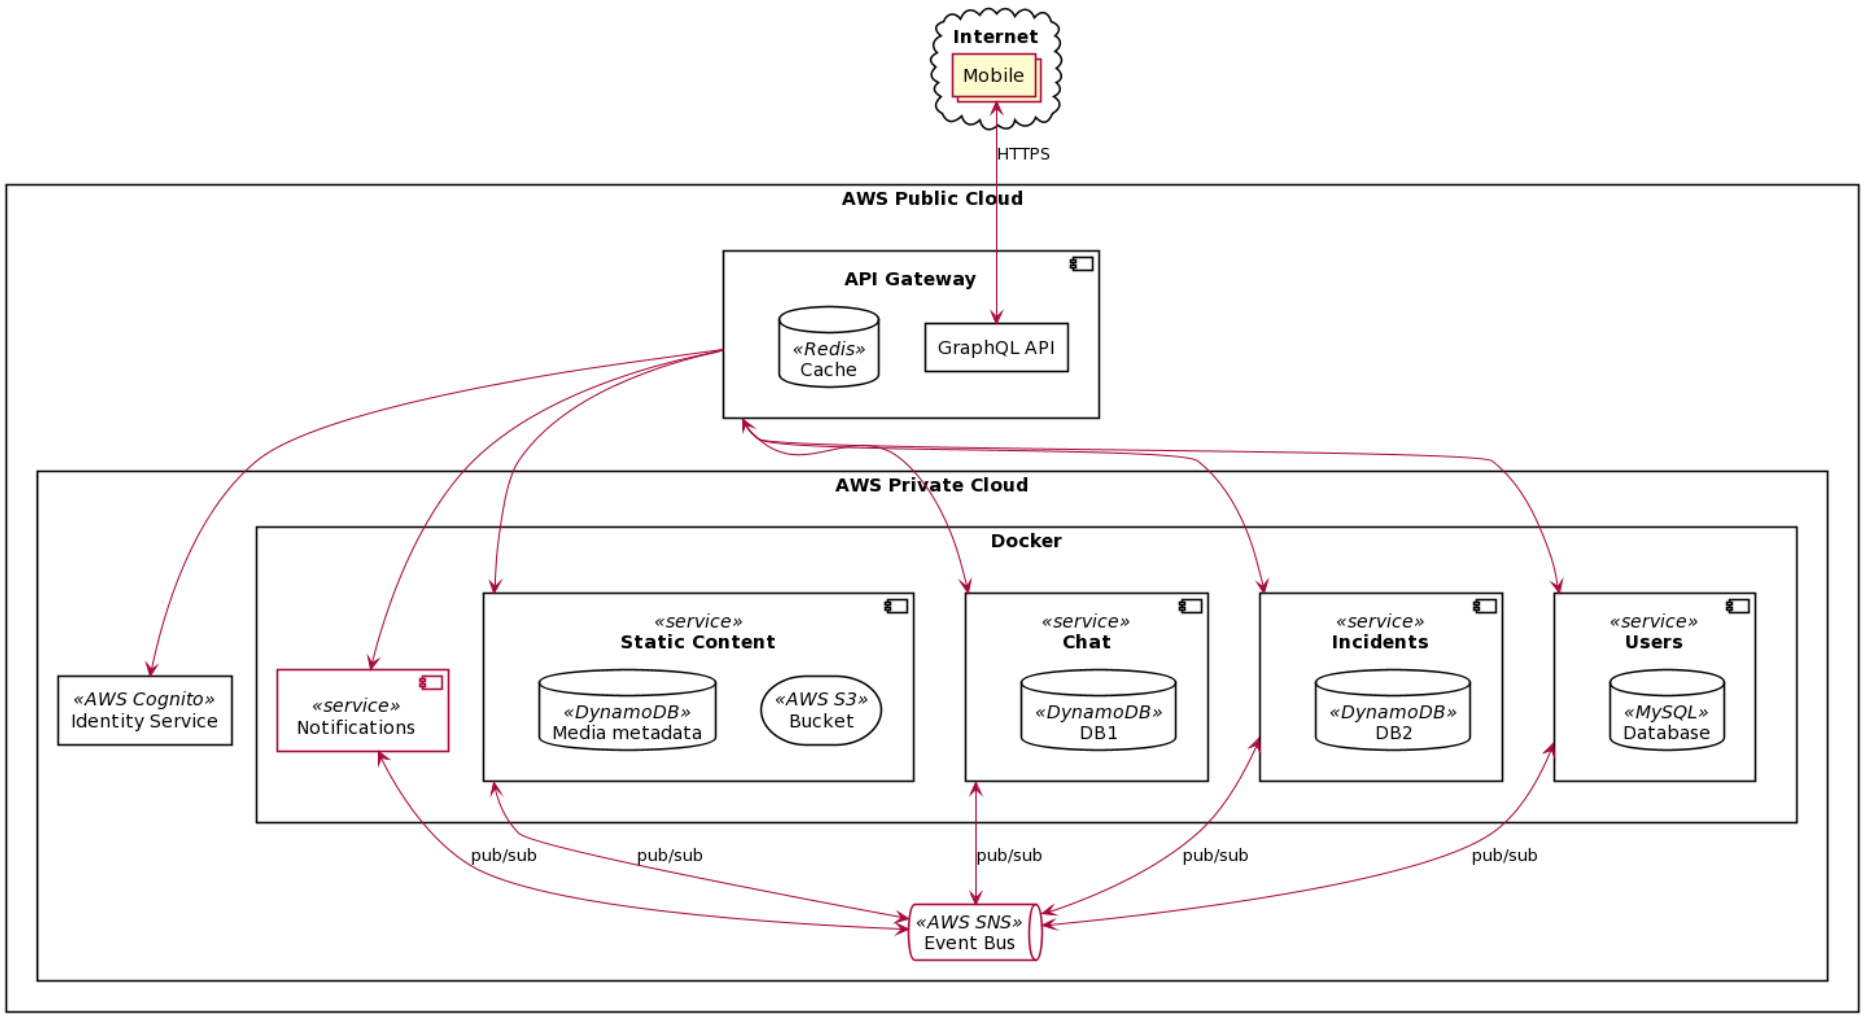
\includegraphics[scale=0.50]{figs/arquitetura.png}
	\label{f.diagrama-arquitetura}
	\legend{\small Fonte: Elaborada pelo autor.}
\end{figure}

\begin{figure}[htbp]
	\caption{\small Visão geral dos eventos assíncronos.}
	\centering
	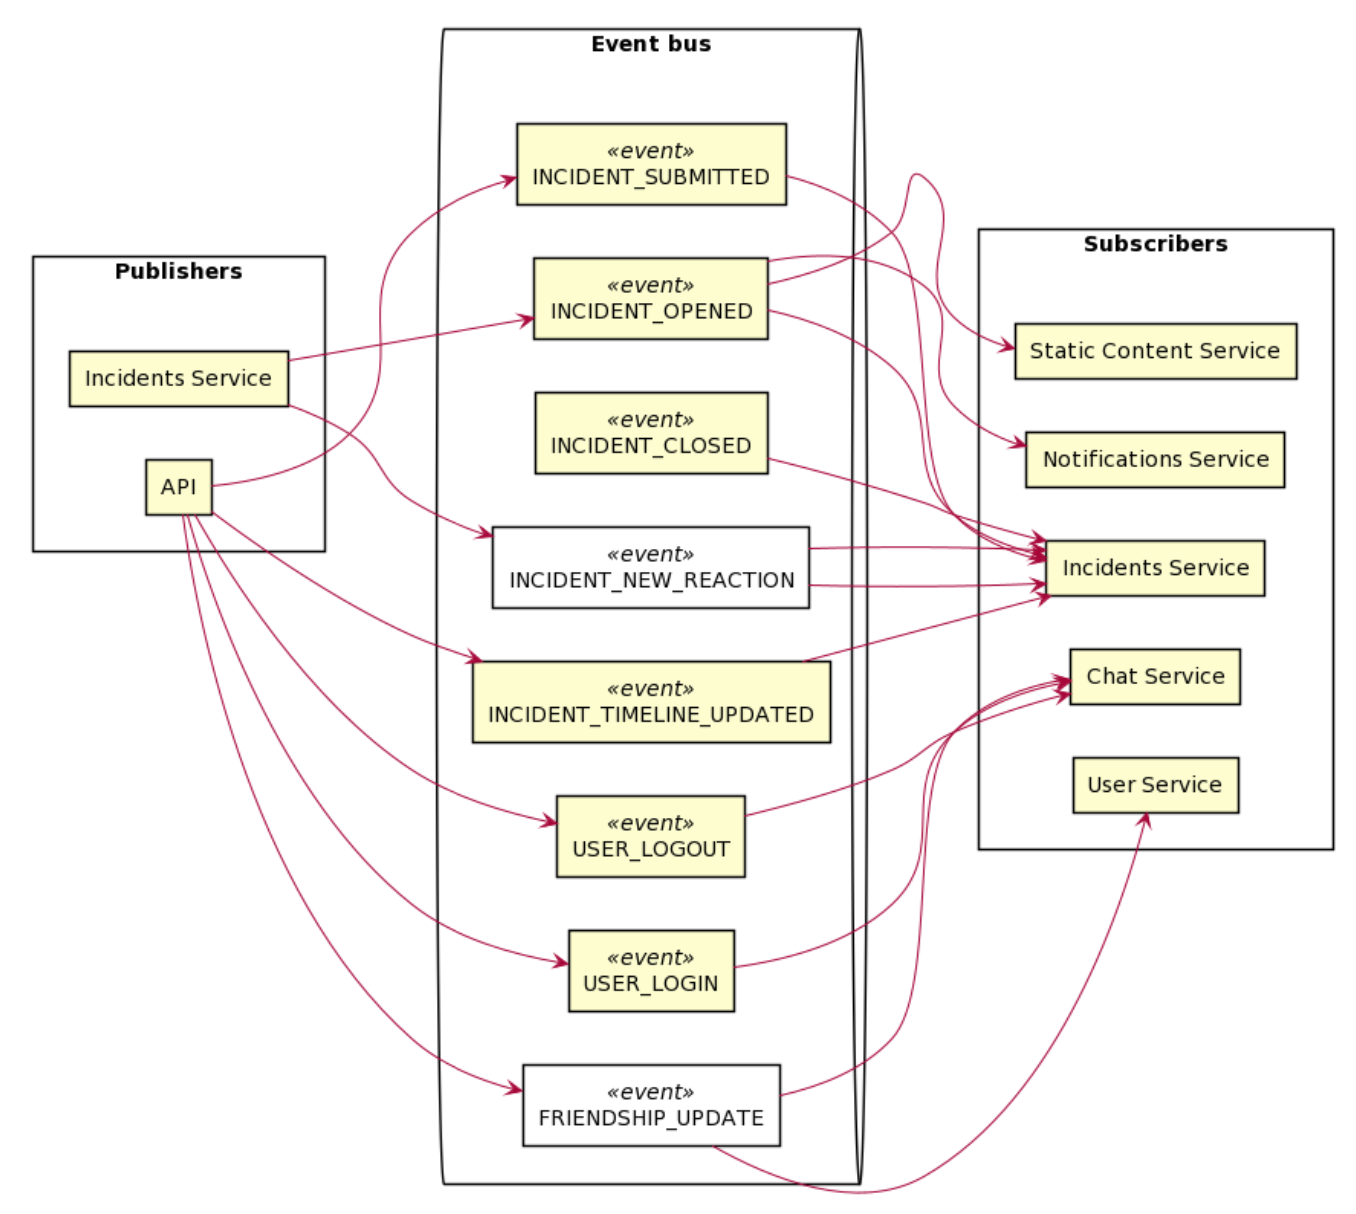
\includegraphics[scale=0.50]{figs/eventos.png}
	\label{f.diagrama-eventos}
	\legend{\small Fonte: Elaborada pelo autor.}
\end{figure}


Abaixo, a figura~\ref{f.diagrama-classes} ilustra as classes que representaram os dados persistidos no banco de dados.

\begin{figure}[htbp]
	\caption{\small Diagrama de classes.}
	\centering
	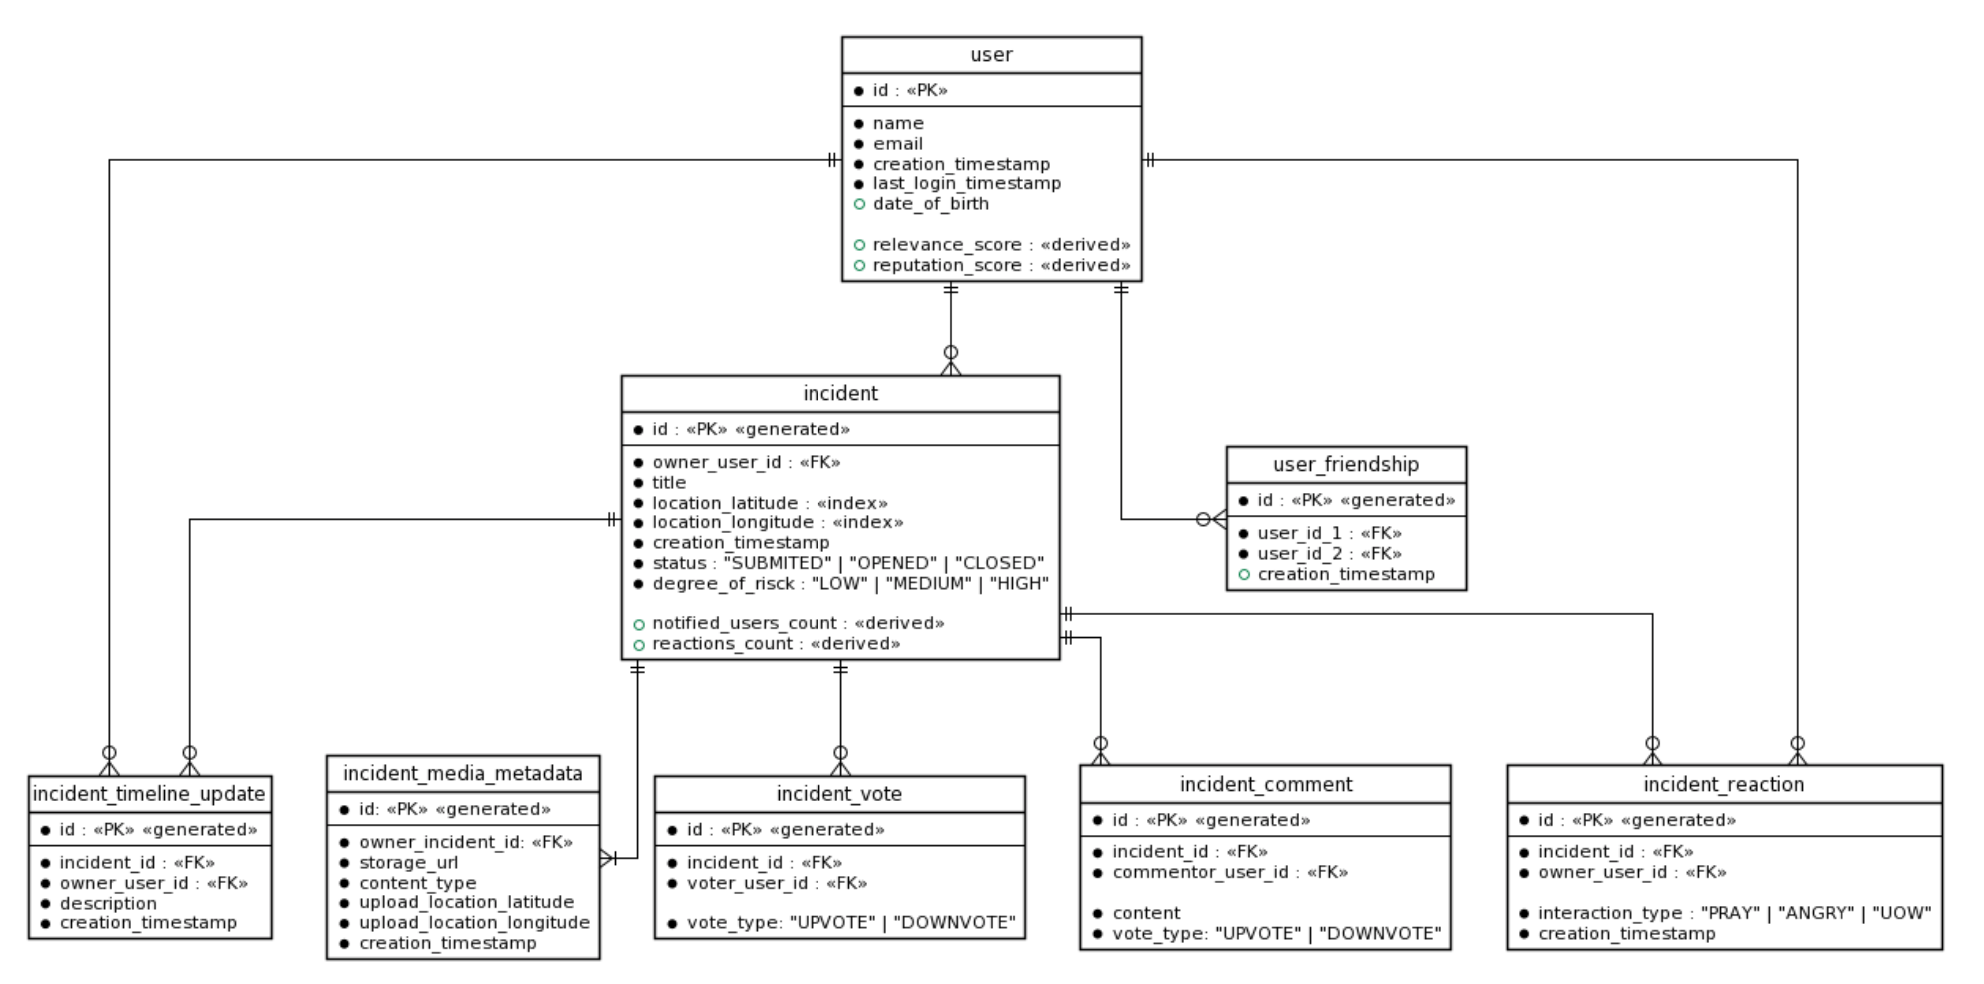
\includegraphics[scale=0.50]{figs/diagrama-de-classes.png}
	\label{f.diagrama-classes}
	\legend{\small Fonte: Elaborada pelo autor.}
\end{figure}

